    Traffic systems in developing-world cities such as Kampala tend to have issues such as limited infrastructure, as well as traffic management resources. Increase in vehicle ownership for both private and personal use among residents in these regions has also played a part in this\cite{gomez-gelvez_modeling_2013}. These factors have an aggregate effect and result in traffic congestion in most of these cities\cite{bashingi_state_2020}.

    One solution that has been put in place in efforts to improve the existing infrastructure is the construction of express highways that use a toll system, and studies have shown that such projects are of great significance spurring economic growth in the region\cite{muvawala_socio-economic_2021}. The highways are less congested and are constructed as alternatives to any already existing routes.Motorists arrive at the tollgates found at the entrance to these roads,pay the toll fees, charged on a vehicle size basis in some cases and are then granted access to the highway.

    Challenges have however risen with this solution, a major one being congestion and queues as motorists wait to pay their toll fees, thus defeating the road’s intended purpose. These challenges can be attributed to issues such as finding cash change as well as limited manpower to attend to the various vehicles accessing the gates\cite{bari_delay_2022}.
    \begin{figure}%
    \centering
    \subfloat[\centering]{{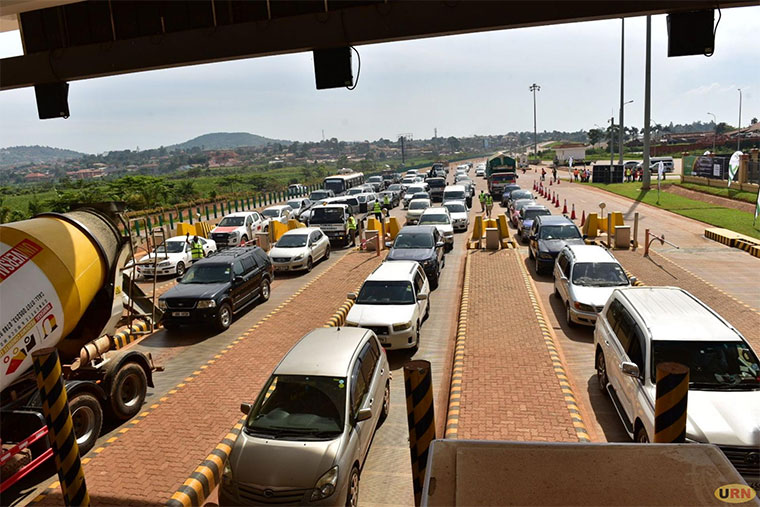
\includegraphics[scale=0.2]{images/ebbs} }}%
    \qquad
    \subfloat[\centering]{{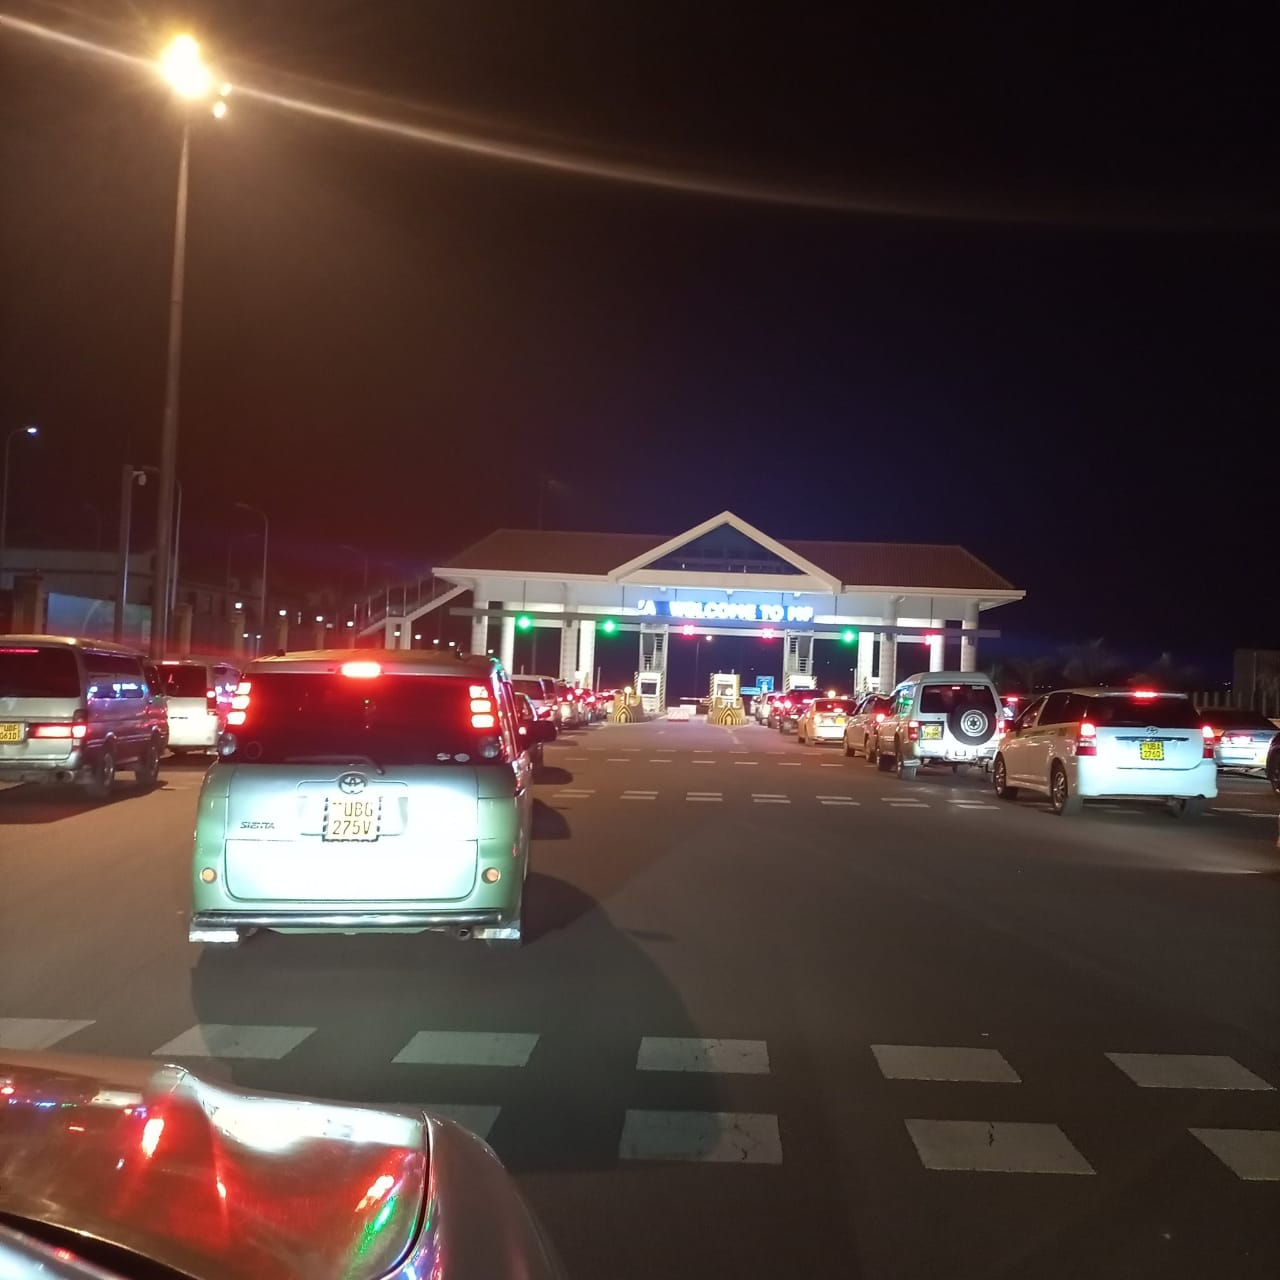
\includegraphics[scale=0.1]{images/ebbs2} }}%
    \caption{Queues at the Entebbe Express Highway}%
    \label{fig:example}%
\end{figure}

    This research therefore explores how techniques from the field of ubiquitous computing can be used along with mobile commerce tools to create a localised low-cost solution to streamline this payment process. Such a system can serve as a demonstration of how intelligent transportation systems can be implemented in Uganda, and in the long run, ultimately aiding in the development of cities like Kampala into smart cities.

    According to Jonathan Reichental, smart cities are a form of Urbanization that leverages technology from a variety of domains such as Internet of Things and cloud computing to improve infrastructure and service delivery, while lowering costs of resource consumption\cite{geng_strategic_2016}. One key feature of such cities is the use of intelligent transportation systems.


    Intelligent Transportation Systems use various technologies to optimise urban mobility guaranteeing safety of drivers\cite{i_meneguette_intelligent_2018}. They use data and communication of various devices, such as sensors embedded inside cars or road side cameras to improve transportation problems in cities.One such technology used in these systems is ubiquitous computing

    Originally coined by Mark Weiser\cite{weiser_hot_1993}, the term ubiquitous computing at its core is concerned with embedding microprocessors into other objects of daily use, connecting them to a given network such as the internet and enabling perform similar tasks for users as normal computers\cite{judith_ubiquitous_2009}. Today, it has a number of applications such as self-driving vehicles, smart devices such like smartwatches and electronic tollgates. With regard to intelligent transportation systems these electronic tollgates can be implemented through the use of ubiquitous computing applications such as use of RFID scanners and tags.These can also be coupled with mobile payment tools to make the entire flow seamless

    Mobile Commerce, on the other hand is a branch of E-Commerce concerned with cashless initiation and verification of payments for goods or services\cite{centellegher_mobile_2018}. In SubSaharan Africa, its commonest implementation has been through the mobile money platforms such as Airtel Money and MTN mobile money. These allow users to easily create accounts using their personal SIM cards and carry out financial transactions such as sending, receiving money or making payments for goods and services\cite{baah_state_2021}.

    \clearpage